\documentclass[conference]{IEEEtran}
\usepackage{cite}
\usepackage{amsmath,amssymb,amsfonts}
\usepackage{algorithmic}
\usepackage{booktabs}
\usepackage{caption}
\usepackage{graphicx}
\usepackage{listings}
\usepackage{textcomp}
\usepackage{xcolor}
\def\BibTeX{{\rm B\kern-.05em{\sc i\kern-.025em b}\kern-.08em
    T\kern-.1667em\lower.7ex\hbox{E}\kern-.125emX}}
\begin{document}


\title{CENG435 Term Project, Part 2\\
}

\author{\IEEEauthorblockN{Doruk Coskun}
\IEEEauthorblockA{
}
\and
\IEEEauthorblockN{Yagmur Oymak}
\IEEEauthorblockA{
}
}

\maketitle

\section{Introduction}

In our CENG435 Term Project Part 2 we have implemented a reliable data transfer protocol on top of UDP in Application layer. To achieve this we have implemented checksum, SEQ counter and timer mechanisms. On top of that, to optimize data transfer rate we have added pipelining and multi-homing strategies. We have implemented Go-Back-N as our pipelining protocol and utilized both links to send data to Destination.

\section{Setting Up the Environment}

In the first part of the assignment we used applications on the routers to forward the packets. In the second part we have set the forwarding tables in the routers. This way the kernel handles the forwarding of packets in the network layer so we got rid of the application layer forwarding scripts. You can check the detailed explanation of how we set the forwarding tables in the README.md file.

We use config files to determine the size of the packets. It can be adjusted through those files. It is important to keep in mind that our packet headers are 20 bytes and the minimum packet size must be larger than that.

We have written our own shell scripts which send the codes to the nodes and set the netem/tc corruption, loss, reorder and delay parameters in the nodes.
Details of how to run the scripts are in the README.md file.

\section{Design Decisions}

In our design, we have decided to implement Go-Back-N protocol and added header to our packets. The size of our headers are 20 bytes in total. The first 4 bytes indicate the SEQ number of the packets and the remaining 16 bytes are used for MD5 Checksum. We have decided that including the packet length to the header was redundant since our Broker and Destination send and read the packets by a predetermined maximum size which is declared in the config file. Packets size less than that do not cause any problems.

When the scripts are executed, 5MB file is sent to Broker from Source over TCP. Broker packages the bytes received from byte stream into packets and sends them to Destination over both routers using UDP. Routers forward the packets to Destination as we have defined in their forwarding tables. Destination expects the packets from both routers. When a packet is received, Destination checks its SEQ number and accepts the packet with the correct SEQ number. When a packet with the expected SEQ number is received, SEQ number counter in Destination is incremented. Regardless whether a packet is accepted or not, an ACK message is sent back to Broker, informing Broker the current SEQ number in the Destination. Broker adjusts its Window according to the SEQ number of the received ACK and sends new packets.

Broker also has a timer. When the timer expires before Broker receives an ACK, it sends the packets in the Window again. Timer is reset and Window is moved if a packet with SEQ number higher than the Base SEQ in Broker is received.

Destination is a synchronized multithreaded application. Sockets which are bound to two different interfaces are run on these threads and awaits packets from different routers. When a packet with expected SEQ number is received, it is written to a file. SEQ number variable is secured with threading lock, preventing concurrent access to the variable by different threads. When a packet is received, regardless of its contents, appropriate ACK packet is sent back, informing Broker about the current SEQ number in the Destination.

Timer in Broker handles the cases where the packets are lost. Our MD5 Checksum mechanism protects against corrupted packets and our SEQ number implementation preserves the integrity of the file when packets are received out of order.

\subsection{Detailed Explanation of Broker Implementation}

Broker is a multiprocess/multithreaded C++ program that was ported from the broker
we had written in C for the first part of the project. Like its predecessor,
it listens a TCP socket for incoming connections from the source. When a connection
is established, it spawns a worker process to handle the connection. Such details
are similar to its predecessor and are already explained in the first report.

The worker process differs greatly, though. First of all, the reason the code was
ported to C++ from C was to borrow as much socket programming code as possible
from the previous implementation, while using high-level threading abstractions of modern C++.

\subsubsection{Packet Structure}
We have a 20 byte header consisting of a 4 byte sequence number and a 16 byte MD5 checksum field.
A packet that is sent from the broker, consisting of not only a header but also a payload
is interpreted as a data packet by the destination. A packet that is sent from
the destination that has no payload (in fact, no packet originating from the destination carry a payload)
is interpreted as an ACK packet by the broker, with the sequence number specified in the header.
A packet originating from the broker with no payload is interpreted as a FIN packet
that is used to signal the end of the transfer. MD5 checksum is used to protect the
integrity of all packets.

\subsubsection{Overview of the Implementation}
As previously mentioned, broker is a multithreaded program.
Separate threads were used to asynchronously read data from the source,
keep track of the timer expiry, send packets to destination and receive ACK packets from
the destination. What follows is a high level overview of the responsibilities of each thread.
\begin{itemize}
    \item
        A thread reads data as byte streams from the source and packetizes the stream.
        It constructs the packet header, appends the payload, computes the checksum and places
        the packet into a synchronized queue. When there is no more data to read
        from the source, it constructs a FIN packet and queues it. Then it
        waits for the ACK handler threads to signal the receipt of the ACK packet
        for that FIN packet. When that ACK is received, it shuts down together with
        the other threads and the worker process exits.
    \item
        To notify timeouts, a SIGALRM handler was used with a period of 50 milliseconds.
        This value was proven experimentally to be sufficiently optimal.
        When the timer expires, the signal handler sets an atomic boolean variable, which is periodically
        checked by a timeout handler thread. When the timeout handler thread is notified of the
        timeout, it resends all packets in the current window.
    \item
        A thread dequeues packets from the aforementioned queue and checks if the
        sender window is full. If it is full, it waits for the window to move, which may
        happen when an ACK packet is received. If it is not, it sends the packet
        through both links\footnote{The reason behind this approach will be explained later.}
        and tries to dequeue the next packet.
    \item
        Two threads wait for ACK packets to arrive, from separate links. When an ACK
        packet is received that frees up space in the sender window, these threads
        are responsible for notifying the sender thread and waking it up.
\end{itemize}
Refer to the comments in the code for detailed explanation of communication and
synchronization of the threads.

\subsubsection{Multihoming}
The broker uses multihoming in order to provide redundancy in high loss or high
corruption scenarios. So, whenever it wants to send a packet to the destination,
it duplicates the packet to both links. This provides a better chance of sending
the packet successfully when there are lots of corrupt or lost packets. We've also
tried another approach to sending separate packets in parallel (using separate threads)
over both links, but our current approach proved to be more than two times faster
in high loss and high corruption scenarios.
The reason is that when there is high loss in the link, it is not beneficial to
send more packets quickly back to back because there will eventually be a lost packet and
the window would have to be resent again. However, if we provide redundancy by sending a
single packet over both links in parallel, we provide redundancy and increase the
reliability this way.

\section{Experiments}

In our experiments we have plotted the results of loss, corruption and reordering tests. We have changed netem/tc properties of the links between Broker and Destination while conducting these tests.
For each property we have plotted three different scenarios.

\subsection{Packet Loss Test}\label{AA}

For the packet loss tests we have set the loss and delay properties of the links as follows:
\begin{itemize}
    \item \textbf{Configuration 1:} 3ms delay and $0.5\%$ loss
    \item \textbf{Configuration 2:} 3ms delay and $10\%$ loss
    \item \textbf{Configuration 3:} 3ms delay and $20\%$ loss
\end{itemize}
For each of the scenarios above, 23 samples were collected.

Table~\ref{table:loss} summarizes our experiment results with 95\% confidence intervals.
Figure~\ref{fig:loss} illustrates the results graphically.
\begin{table}
    \centering
    \begin{tabular}{c c c c}
        \toprule
        NetEm loss & $\mu$ & $\sigma$ & Error \\
        $0.5\%$   &   $97.1s$   &   $1.4s$    &   $0.572s$ \\
        $10\%$   &    $294s$   &   $6.68s$    &   $2.73s$ \\
        $20\%$   &    $559s$   &   $17s$    &   $6.95s$ \\
        \bottomrule
    \end{tabular}\label{table:loss} \\
    \caption{Summary of packet loss experiment results}\label{table:loss}
\end{table}

\begin{figure}
    \centering
    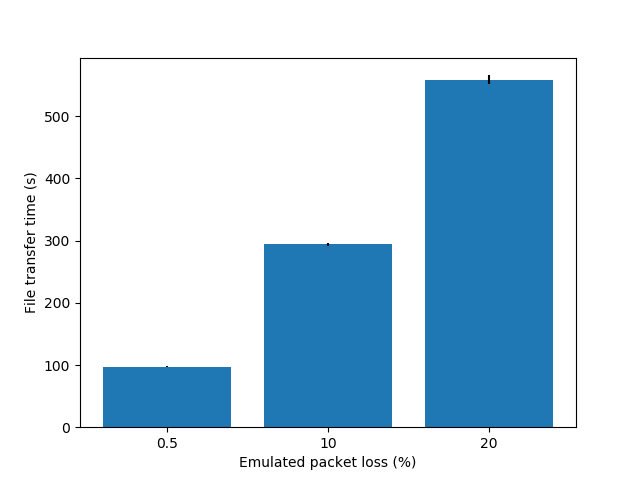
\includegraphics[scale=0.6]{graphics/plot-loss}
    \caption{Emulated loss vs.\ file transfer time}\label{fig:loss}
\end{figure}

\subsection{Packet Corruption Test}\label{AA}

For the packet corruption tests we have set the corruption and delay properties of the links as follows:
\begin{itemize}
    \item \textbf{Configuration 1:} 3ms delay and $0.2\%$ corruption
    \item \textbf{Configuration 2:} 3ms delay and $10\%$ corruption
    \item \textbf{Configuration 3:} 3ms delay and $20\%$ corruption
\end{itemize}
For each of the scenarios above, 23 samples were collected.

Table~\ref{table:corruption} summarizes our experiment results with 95\% confidence intervals.
Figure~\ref{fig:corruption} illustrates the results graphically.
\begin{table}
    \centering
    \begin{tabular}{c c c c}
        \toprule
        NetEm corruption & $\mu$ & $\sigma$ & Error \\
        $0.2\%$   &   $89.5s$   &   $0.597s$    &   $0.249s$ \\
        $10\%$   &    $195s$   &   $7.04s$    &   $2.94s$ \\
        $20\%$   &    $446s$   &   $15.5s$    &   $6.48s$ \\
        \bottomrule
    \end{tabular}\label{table:corruption} \\
    \caption{Summary of packet corruption experiment results}\label{table:corruption}
\end{table}

\begin{figure}
    \centering
    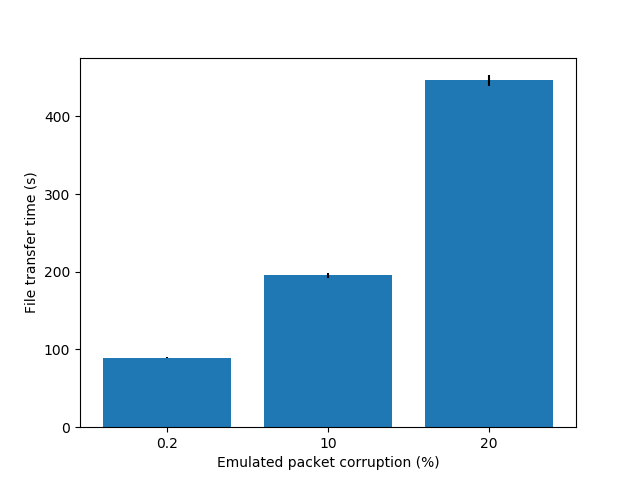
\includegraphics[scale=0.6]{graphics/plot-corruption}
    \caption{Emulated corruption vs.\ file transfer time}\label{fig:corruption}
\end{figure}

\subsection{Packet Reordering Test}\label{AA}

For the packet reordering tests we have set the reorder and delay properties of the links as follows:
\begin{itemize}
    \item \textbf{Configuration 1:} 3ms delay and $1\%$ reorder
    \item \textbf{Configuration 2:} 3ms delay and $10\%$ reorder
    \item \textbf{Configuration 3:} 3ms delay and $35\%$ reorder
\end{itemize}
For each of the scenarios above, 22 samples were collected.

Table~\ref{table:reorder} summarizes our experiment results with 95\% confidence intervals.
Figure~\ref{fig:reorder} illustrates the results graphically.
\begin{table}
    \centering
    \begin{tabular}{c c c c}
        \toprule
        NetEm reorder & $\mu$ & $\sigma$ & Error \\
        $1\%$   &   $89.3s$   &   $0.004s$    &   $0.002s$ \\
        $10\%$   &    $89.5s$   &   $0.36s$    &   $0.148s$ \\
        $35\%$   &    $99.8s$   &   $12.8s$    &   $5.35s$ \\
        \bottomrule
    \end{tabular}\label{table:reorder} \\
    \caption{Summary of packet reordering experiment results}\label{table:reorder}
\end{table}

\begin{figure}
    \centering
    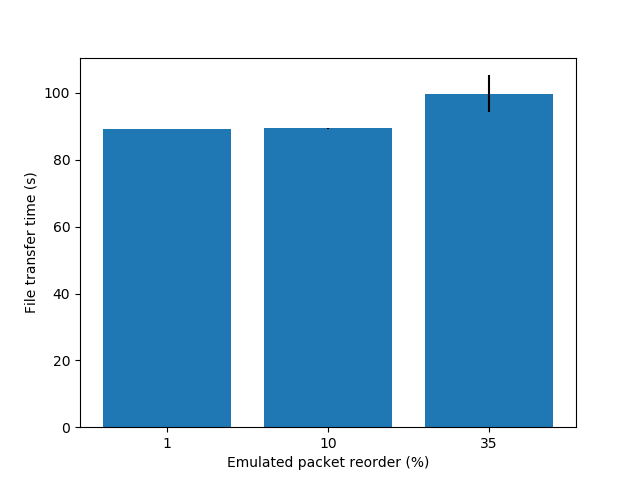
\includegraphics[scale=0.6]{graphics/plot-reorder}
    \caption{Emulated reordering vs.\ file transfer time}\label{fig:reorder}
\end{figure}

\end{document}
